%!TEX root = ../dissertation.tex
\chapter{Experiments}

All of the following experiments were executed on a MacBook Air with a 1.4 GHz Intel Core i5 processor and 8GB of RAM.
This is a very basic setup and just further goes to show the potential ubiquity of using discrete optimization techniques.
Our algorithm is run on one of the training folds of the COMPAS dataset.
The fold has 6489 data points from which we're able to extract 155 rules.
2947 of these individuals are labeled "yes", meaning they have committed a second crime after being arrested---the other 3542 individuals are labeled "no".

Naively evaluating all prefixes of up to length length 5 would require examining 84,382,025,575 different prefixes.
However, with our solution, we examine only 99,891,878 prefixes in total.
This is a reduction of 845x.
Note that this is a lower bound since any brute force solution would have to examine prefixes of longer than length 5 in order to certify optimality.
It takes us 0.000002s to evaluate a single prefix.
Thus, a naive solution would take 168,764s---about 2 days.
While this is a long time, it is still not a completely unreasonable amount of time, though it clearly wouldn't scale to larger problems.

However, if we look at how processor speeds have changed over the last 25 years, we can see that computers are about 1,000,000 faster now than they were in 1993. \cite{Supercomputer}
Thus, when we combine our algorithmic improvements with the increased processor speeds, we see that our algorithm runs almost 1 billion times faster than a naive implementation would have in 1993.
%Nov 2016 125,435.9 TFlops/s
%June 1993 131.0 GFlops/s
This explains why there has been a dearth of work on algorithms focused on optimality.

We first examine how much each of our optimizations helps.
We will show that without our algorithmic and data structure improvements, it would be intractable to solve a real-world problem.
We will also show that even with our improvements, this algorithm would not have been able to be run just 25 years ago.
Next, we will examine the improvements made to our symmetry-aware map to reduce the memory overhead on our algorithm.
Finally, we will explore a parallel implementation.

\begin{figure}[t!]
%\vspace{-3mm}
\begin{algorithmic}
\normalsize
\State \bif $(age=23-25) \wedge (priors=2-3)$ \bthen $yes$
\State \belif $(age=18-20)$ \bthen $yes$
\State \belif $(sex=male) \wedge (age=21-22)$ \bthen $yes$
\State \belif $(priors>3)$ \bthen $yes$
\State \belse $no$
\end{algorithmic}
%\vspace{-3mm}
\caption{An example rule list that predicts two-year recidivism for the COMPAS dataset, found by CORELS.}
\label{fig:rule-list}
\end{figure}

\section{Ablation--how much does each bound/optimization help?}

We wished to determine how much each theoretical bound and data structure optimization helped, so that we could determine which one was the most helpful.
In addition, we wanted to find out how much of an overall speed-up our work has given us.
In order to do that, we ran a number of experiments where we took out a single component from our system and measured the effects on the runtime and memory usage of our algorithm.
We find that the equivalent points bound is our most important optimization for running in a reasonable amount of time.
Each other optimization and bound plays an important, but not crucial, role in the speed of our algorithm.

\subsection{Full CORELS system}

Our baseline system with all of our improvements is the CORELS system.
Running the full CORELS system on the COMPAS dataset yields the optimal solution and its certificate within 121s.
The maximum memory usage is 150MB, with the majority of that coming from our prefix trie.

\begin{figure}[t!]
\begin{center}
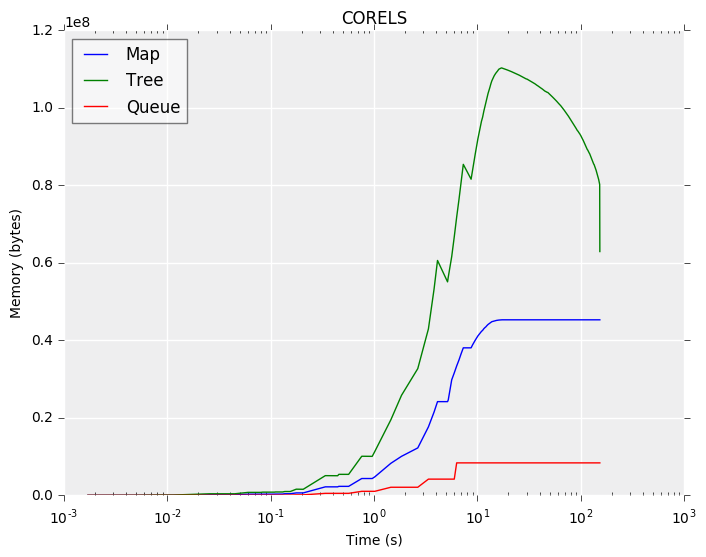
\includegraphics[width=0.4\textwidth]{figs/corels_mem.png}
\end{center}
\caption{Memory usage of full CORELS system. Our prefix tree accounts for the bulk of the memory usage}
\label{fig:corels-mem}
\end{figure}

With about 1 million items active at the peak, this comes out to about 150 bytes per item.
This includes copies of that item that are kept across the prefix trie, symmetry-aware map, and queue.

\begin{figure}[t!]
\begin{center}
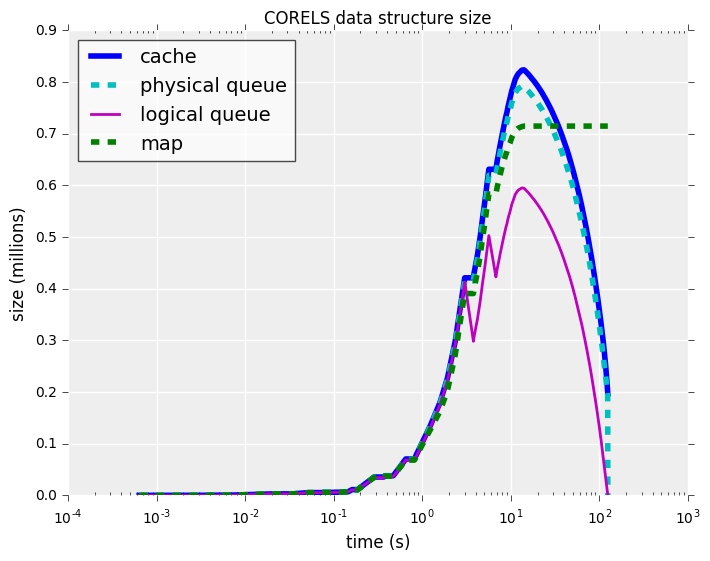
\includegraphics[width=0.4\textwidth]{figs/corels_size.png}
\end{center}
\caption{The size (in number of items) of each of our main data structures. Corresponds to the amount of memory used, as shown above.}
\label{fig:corels-size}
\end{figure}

\begin{figure}[t!]
\begin{center}
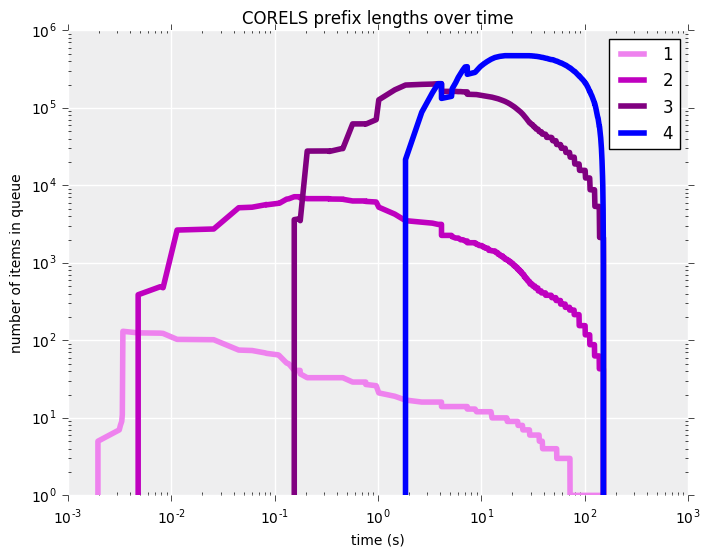
\includegraphics[width=0.4\textwidth]{figs/corels_prefixes.png}
\end{center}
\caption{Tracks the number of prefixes of a given length active in the queue for the full CORELS system}
\label{fig:corels-prefixes}
\end{figure}

\subsection{Priority Queue} \label{exp:priority}

One of our first optimizations was the use of a priority queue to utilize different exploration techniques. 
Removing the priority queue and simply using BFS allows us to find the optimal solution and certificate in 142s.
So, the queue gives us a slight speed-up without requiring much memory at all.
On other problems, we've found that using a priority queue can lead to a large speed-up.

\subsection{Support Bounds}

The support bounds are intrinsic to the rules and are the first bounds we check in our execution because they are the simplest to compute.
This ease of computation belies the fact that these bounds prevent the pursuit of useless rules.
Without these bounds we complete the certification in 261s.

\subsection{Symmetry-aware map}

The symmetry-aware map is a novel way of approaching branch-and-bound and it plays a large role in our elimination of search space.
Using the symmetry-aware map means that we are able to only pursue one prefix out of all of its permutations.
As our prefixes grow to length 4 and beyond, that means we can eliminate at least 23 prefixes.
This is an important optimization and removing it takes a long time to complete the certification---1147s.

\begin{figure}[t!]
\begin{center}
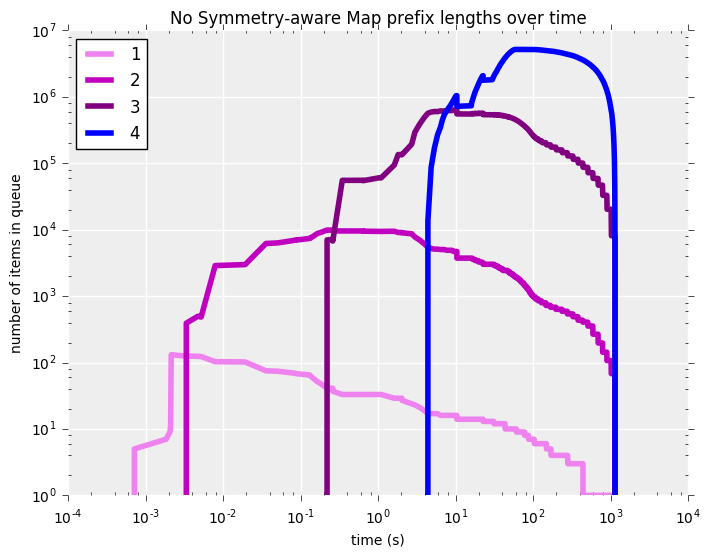
\includegraphics[width=0.4\textwidth]{figs/pmap_prefixes.png}
\end{center}
\caption{Tracks the number of prefixes of a given length active in the queue for CORELS without a symmetry-aware map}
\label{fig:pmap-prefixes}
\end{figure}

\subsection{Lookahead Bound}

Our lookahead bound is useful for preventing us from examining longer prefixes than we need to.
From running our full CORELS system, we know that our optimal rule list is of length 4.
With our lookahead bound, we never have to examine prefixes of length 5.
However, removing that bound means that we do look at many prefixes of length 5 which drastically slows our computation to 2360s.

\begin{figure}[t!]
\begin{center}
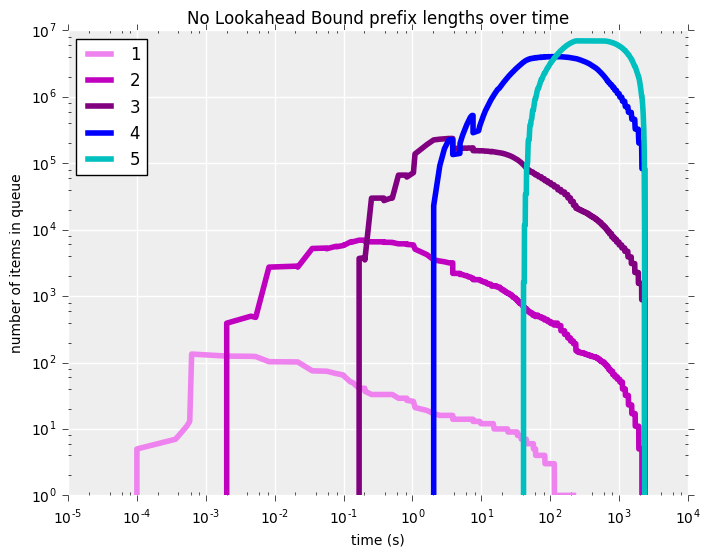
\includegraphics[width=0.4\textwidth]{figs/lookahead_prefixes.png}
\end{center}
\caption{Tracks the number of prefixes of a given length active in the queue without our lookahead bound}
\label{fig:lookahead-prefixes}
\end{figure}

\subsection{Equivalent points bound}

The equivalent points bound is our optimization that provides the largest benefit.
Since all of our other bounds eliminate prefixes contingent on the lower bound, the equivalent points bound is important because it tightens the lower bound.
Removing this bound makes it impractical to complete real world problems.
We stop execution after multiple hours (8500 s) and show that there is still a large portion of the search space to be explored.

\begin{figure}[t!]
\begin{center}
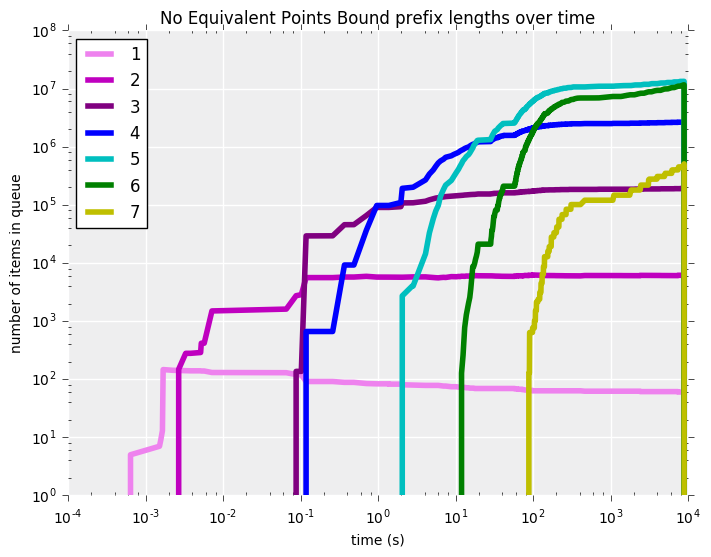
\includegraphics[width=0.4\textwidth]{figs/equivalent_prefixes.png}
\end{center}
\caption{Tracks the number of prefixes of a given length active in the queue without the equivalent points bound}
\label{fig:equivalent-prefixes}
\end{figure}

TODO: Re-run BFS because numbers seem wrong

\begin{table}[t!]
\begin{tabular}{l | c | c | c | c | c}
Removed component & $t_\text{total}$ (s) & $t_\text{opt}$ (s) & $i_\text{total}$ ($\times 10^6$) & $Q_\text{max}$ ($\times 10^6$) & $K_\text{max}$ \\
\hline
none (CORELS) & 121 & 7.3 & 0.83 & 0.59 & 4 \\
priority queue (BFS) & 142 & 0.14 & 0.73 & 0.19 & 5 \\
support bounds & 261 & 11 & 1.3 & 0.98 & 4 \\
symmetry-aware map & 1147 & 23 & 6.5 & 5.6 & 4 \\
lookahead bound & 2360 & 7.6 & 7.6 & 10.7 & 5 \\
%equiv. pts. bound & 188.6 (104.6) & 6178 (1840) & 803.8 (0.1) & 790.5 (0.4) & 10-10
equivalent pts bound & $>$8500 & $>$42 & $>$29 & $>$28 & $\ge$7
\end{tabular}
\vspace{4mm}
\caption{Per-component performance improvement.
%
The columns report total execution time,
time to optimum, number of queue insertions,
maximum queue size, and maximum evaluated prefix length.
%
The first row shows CORELS; subsequent rows show variants
that each remove a specific implementation optimization or bound.
%
(We are not measuring the cumulative effects of removing a sequence of components.)
%
All rows represent complete executions, except for the final row,
in which each execution was terminated due to memory constraints
}
\label{tab:ablation}
\end{table}

\section{Symmetry-aware Map Optimization}

As one of our two main data structures, the memory usage of our symmetry-aware map is something that was very important to us.
We saw above that running without a symmetry-aware map leads to a much longer runtime, so it was crucial that we cut down on this overhead.
We initially found that we often had trouble running large data sets because we would run out of memory before certifying the optimal rule list.
In these long runs, our permutation map would grow to be hundreds of thousands or millions of entries large.
Thus, carrying a lot of memory overhead with each node led to serious memory bloat and ran us out of memory.
This section explores some of the techniques we used to handle this memory bloat.

Our symmetry-aware map was originally an STL map with keys as STL sets of size\_t and values as pairs of STL vectors of size\_t and a double.
The first problem is that the STL map is implemented as a red-black tree, meaning every node had the overhead of multiple pointers pointing to its children.
This can be solved using a STL unordered map, which is implemented as a hashtable.
That has some overhead, since it will allocate more buckets than are filled, but nowhere near to the two pointers per node of overhead of the STL map.

Next, the representation of the rule ids no longer had to be size\_t.
We made an assumption that we'll never have more than 65000 rules, so we used unsigned shorts for our rule ids.
This means that our final data structure was able to use only 2 bytes per rule id instead of 8 bytes for a size\_t.
Since we're keeping two different representations of the prefix--the canonical order and the actual order of the prefix, and these prefixes can be of length on the order of 5 rules, saving 6 bytes per rule translates to a lot of 

Our initial implementation used an STL set as the key, which carries a lot of overhead because of all the operations that a set needs to support.
For a prefix of length 6, the corresponding key therefore takes up 
After starting with the STL set, we transition to a sorted STL vector.
This reduced overhead because a vector is essentially just an array with a little bit of overhead.
However, all of these STL containers support a broader range of operations than we needed.
All we needed was some way to compare the canonical orders and determine if they were the same.
We eventually achieved this simply by allocating a chunk of memory that held the length of the prefix and the sorted order of the ids.
This means that, for a prefix of length 6, we use 14 bytes for the key.

We had a similar set of issues with our values for the permutation map.
Beginning with a STL vector to keep track of the actual order of the rules in the prefix, we again wanted to remove the overhead incurred by the fact that STL containers need to support a wider array of operations than we needed.
Thus, we could use a similar technique to what we did with the keys to keep track of the prefix order.
However, in fact, we can do even better because we already have a canonical representation of the rules--all we need in the value was the ordering of those rules.
Thus, we can use unsigned chars instead of unsigned shorts to record the index of where the rules in the canonical order are in the prefix.

\begin{table}[t!]
\begin{tabular}{l | c | c | c | c }
Map version & Key version & Value version & Total Memory (b) & $t_\text{total}$ (s)\\
\hline
Map & Set (size\_t) & Vector (size\_t) & 190751744 & 154 \\
Unordered Map & Set (size\_t) & Vector (size\_t) & 185897576 & 150 \\
Unordered Map & Set  (unsigned short) & Vector (unsigned short) & 148611880 & 148 \\
Unordered Map & Vector (unsigned short) & Vector (unsigned short) & 68713960 & 147 \\
Unordered Map & Custom Key & Custom Value & 62865376 & 139 \\
\end{tabular}
\vspace{4mm}
\caption{Symmetry aware map improvements.
%
The columns report the type of map,
type of key, type of value,
total memory used by the symmetry-aware map, and time of execution.
%
Each row represents a different version of the symmetry aware map that we tested.
We see that 
}
\label{tab:pmap}
\end{table}

In total, these improvements give us a 3x memory reduction on this problem.
This takes the permutation map from being the largest data structure to being smaller than the tree.
On larger problems, this memory decrease is even more important.

However, these optimizations all pertained to the symmetry-aware map with prefix keys.
Dealing with the captured vector keys required a different approach.
Our captured vectors were of type mpz, and since unordered\_map requires a custom hash for unsupported types, we had to find a way around that.
STL has some hash functions for built in types, so we initially wrote a function to convert between our VECTOR type and a $std::vector<bool>$.
This conversion turned out to be very slow, especially as we were running on data sets with many samples, meaning these mpz types were fairly memory intensive.
Once we wrote our own hash function and were able to use our mpz type again, it became much faster.

\section{Parallelization}

The majority of the time of our program is spent in the incremental section of our execution.
Trying to extend prefixes by calculating the bounds and inserting into our various data structures is the vast majority of our program.

So, we began by trying to parallelize the inner loop of our incremental evaluation.
This inner loop involves trying to add all possible rules to the prefix we're currently trying to extend.
In order to add these rules, though, we need to calculate the bounds based on characteristics of the parent prefix.
Without locking the parent, we run into a race condition that leads to a segfault in the STL code.
Locking the parent had too much contention, however, because all of our threads needed to own the parent lock for the majority of the loop---essentially rendering the loop sequential.

We realized, however, that the tree structure of our prefix trie lends itself nicely to parallelization.
Instead of parallelizing the evaluation of a single prefix, we can parallelize our search over the tree itself.
We do this by creating the tree in the master thread and then spawning worker threads to work in different parts of the tree.
Thus, there is no contention on parents since only one thread can access a node at a time.
The shared state only consists of the minimum objective, and this is kept in the master thread.
Deletion and garbage collection is handled by the master thread as well.

We find a linear speed up when moving from 1 to 2 threads, but diminishing returns as we increase the number of threads.